\section{A reproducible planning evaluation}
\label{sec:C10:evaluation}
The evaluation record should contain the initial environment, interpreted goal, available tools, permissions, plan representation, observation policy, execution budget, and acceptance criterion. Baselines should include direct reactive control, a fixed decomposition, replanning without persistent reflection, and the proposed planning method. When a world model or verifier is added, hold the downstream policy fixed in a mechanistic ablation and also report a separately tuned system comparison. This separates component attribution from the practical performance of the complete integration.

Measure more than final success. Record invalid actions, violated preconditions, unnecessary operations, recovery success, corruption of initially correct artifacts, and the number of opportunities for irreversible effects. Use task-level paired comparisons and repeated runs where stochasticity is material. Preserve failures and censored runs in denominators. A planner that completes fewer tasks but avoids prohibited actions may satisfy a different operating objective from one that maximizes unconstrained success; the comparison must state that objective before ranking them.

The execution pattern can be stated as a guarded state recurrence. Let $s_0=\mathcal R(H_0,o_0)$ reconcile recorded history with a current observation $o_0$, and let $B_0$ be the admitted resource budget. At iteration $n$, a plan-proposal law $\Pi$ and prefix selector $\alpha$ produce
\begin{equation}
 p_n\sim\Pi(\cdot\mid s_n,B_n),\qquad
 a_n=\alpha(p_n,s_n)\in\mathcal A\cup\{\bot\}.
\label{eq:C10:plan-prefix}
\end{equation}
The selector returns the next primitive operation of a prefix whose modeled preconditions hold, or $\bot$ when the next operation is unresolved. Let $\mathcal D$ acquire the required evidence and let $\mathcal E_{\nu_n}$ dispatch under the authority epoch current at execution. An observed-result update $\mathcal U$ retains actual evidence. The predicate $q(y)\in\{0,1\}$ identifies a partial or unknown outcome when it equals one; $\mathcal H$ augments that state with a proposed recovery plan:
\begin{equation}
\begin{aligned}
 y_n&=
 \begin{cases}
 \mathcal D(s_n),&a_n=\bot,\\
 \mathcal E_{\nu_n}(a_n,s_n),&a_n\ne\bot,
 \end{cases}\\
 s_n^+&=\mathcal U(s_n,y_n),\\
 s_{n+1}&=
 \begin{cases}
 \mathcal H(s_n^+,y_n),&a_n\ne\bot,\ q(y_n)=1,\\
 s_n^+,&a_n=\bot\ \vee\ q(y_n)=0,
 \end{cases}\\
 B_{n+1}&=B_n-\rho_n.
\end{aligned}
\label{eq:C10:observed-transition}
\end{equation}
The charge $\rho_n\geq0$ includes the complete iteration, including evidence acquisition and recovery planning. The operators use realized observations; a predicted tool result does not substitute for $y_n$. A recovery proposal is retained work to evaluate, not evidence that compensation has executed.

Let $g(s)\in\{0,1\}$ be the specified goal-checker verdict and $b(s,B)\in\{0,1\}$ the resource-sufficiency verdict for safe continuation. With the latter checked after each completed transition, termination and reporting are
\begin{equation}
\begin{aligned}
 \tau_g&=\inf\{n\geq0:g(s_n)=1\},\\
 \tau_b&=\inf\{n\geq1:b(s_n,B_n)=0\},\\
 \tau&=\min\{\tau_g,\tau_b\},\\
 \mathcal O_\tau
   &=\bigl(\mathcal C^+(s_\tau),\mathcal C^?(s_\tau)\bigr),
   \qquad \tau<\infty.
\end{aligned}
\label{eq:C10:plan-stop-report}
\end{equation}
Here $\mathcal C^+$ collects verified outcomes with their evidence, including verified failures, and $\mathcal C^?$ retains unresolved outcomes. Initial admission and finite termination require their own implementation conditions. Neither the operator names nor a positive goal verdict establish properties beyond the checker's scope. Every predicate and update needs an implementation and tests against the actual environment.

Planning and self-correction improve agent behavior when they connect hypotheses to observed state and retain the evidence needed to revise them. Their failure modes are equally concrete: a wrong goal, an aliased belief, an invalid local contract, a misleading critic, a stale skill, or an unrecognized partial effect. Treating these as distinct mechanisms permits stronger analysis than attributing all outcomes to an undefined capacity for deliberation. It also connects planning to the rest of the system: context supplies the current evidence, memory supplies prior cases, the policy proposes actions, and execution determines what actually becomes true.

\paragraph{A temporal precondition counterexample.}
Consider a plan that reads a record at version seven, computes an update, and writes it after another actor has committed version eight. The read establishes the precondition only at observation time. If the write ignores the version, a locally well-formed plan can overwrite new information. An execution-time compare-and-swap condition changes the operation semantics: the write succeeds only if the version remains seven, otherwise the planner receives a conflict and must re-read or reconcile. This example shows why a correct textual deduction from a stale premise does not establish a valid external transition.

The same pattern appears with authorization. A permission observed during planning may be revoked before execution. A hard boundary checks the current authorization epoch, while the planner treats denial as new state information. Retrying the identical operation without refreshing that state is not self-correction. A learned policy can decide how to adapt after denial, but should not be allowed to reinterpret denial as permission because it believes the task is important. The separation of model inference and authoritative execution is what makes this behavior testable.

For multi-step plans, attach a state version or relevant precondition set to each consequential operation. A version mismatch does not always require discarding the entire plan: independent earlier conclusions may remain valid. The planner can maintain a dependency graph and invalidate only artifacts whose premises changed, provided that dependency relation is complete for the claimed reuse. Incomplete dependencies create the same kind of silent stale-state error as invalid KV reuse. Conservative full replanning costs more but supplies a useful reference baseline for evaluating selective invalidation.

A controlled test introduces concurrent updates at predetermined points while keeping the model and task fixed. Compare blind execution, full replanning after every change, and dependency-aware replanning. Measure lost updates, unauthorized attempts, useful work retained, observation cost, and complete task latency. These are proposed experiments; no result is presumed. The event schedule should be hidden from the agent but retained by the evaluator, and each run should start from a reproducible environment snapshot. Randomized schedules can test robustness after deterministic cases establish basic correctness.

This temporal view also improves self-correction evaluation. A revision that was correct when generated can become invalid before acceptance, while an apparent regression can reflect a changed task state rather than worse reasoning. Preserve the state against which each candidate and feedback item was judged. Without that association, a system can learn contradictory lessons from the same artifact or report a false improvement by comparing outcomes under different environments. State-indexed evidence is therefore a prerequisite for interpreting planning progress across long sessions, concurrent agents, and tool upgrades.


Figure~\ref{fig:C10:versioned-precondition} isolates the mechanism and its stated information boundaries.
\begin{figure}[!htbp]
\centering
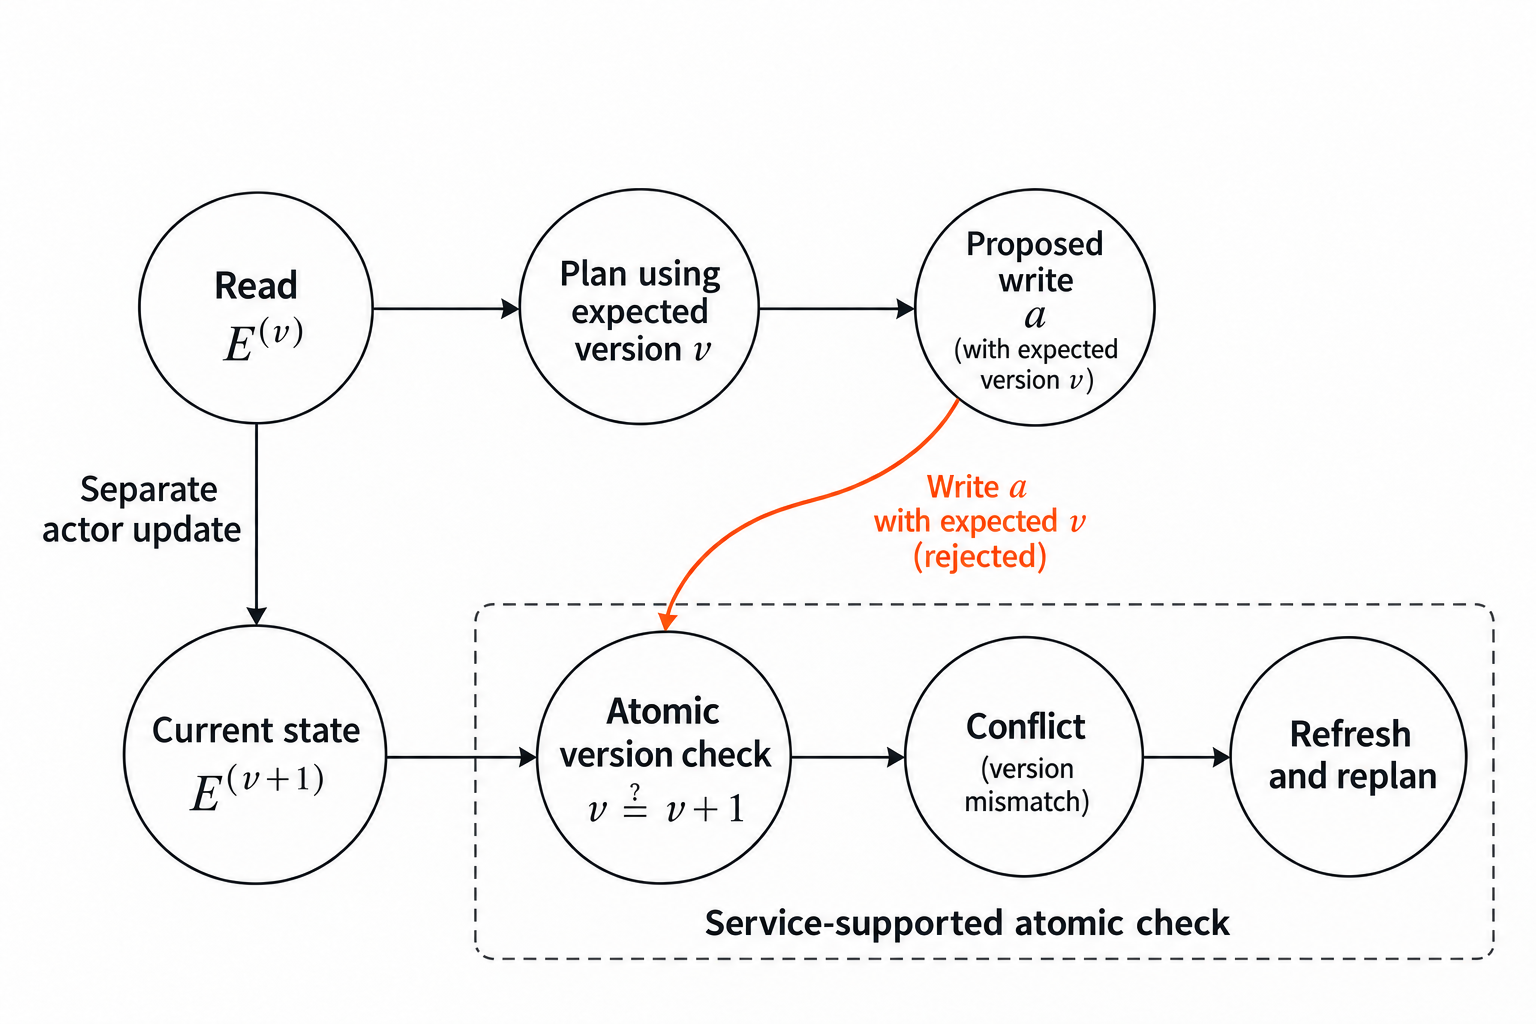
\includegraphics[width=\linewidth]{book/figures/assets/F10review.png}
\caption{An observation-time precondition can become stale before execution. Here an intervening update changes version $v$ to $v+1$, so a service-supported atomic expected-version check rejects the proposed write. The planner must refresh or reconcile. This original mechanism example does not attribute atomicity to an ordinary client-side check.}
\label{fig:C10:versioned-precondition}
\end{figure}
